\documentclass{beamer}

%\usepackage{graphicx}
%\usepackage{tikz}
%\usepackage[absolute,overlay]{textpos}
%\usepackage{listings}
%\usepackage{textpos}
\usepackage{graphicx}


%\includeonlyframes{1,2,3}


\usetheme{Antibes}
% Orange
\usecolortheme[RGB={233,100,35}]{structure}

\usebackgroundtemplate{
    % UniCT Logo
    
\includegraphics[width=370pt]{img/unict.jpg}
}

\newtheorem{samplecode}{Sample Code}

%\setbeamercovered{transparent}
\setbeamertemplate{footline}[frame number]{}
\setbeamertemplate{blocks}[rounded][bg=red]

\newcommand{\tildett}{\raise.17ex\hbox{$\scriptstyle\mathtt{\sim}$}}
% Spaces
\newcommand{\N}{\vskip 0.3 cm}
\newcommand{\n}{\vskip 0.2 cm}
\newcommand{\TAB}{\hskip 1.8 cm}
\newcommand{\tab}{\hskip 0.6 cm}

% Colors
\newcommand{\red}[1]{\textcolor[rgb]{.8,0,0}{#1}}
\newcommand{\blue}[1]{\textcolor[rgb]{0,0,.7}{#1}}
\newcommand{\navy}[1]{\textcolor[rgb]{0,0,.5}{#1}}
\newcommand{\purple}[1]{\textcolor[rgb]{.7,0,.8}{#1}}
\newcommand{\green}[1]{\textcolor[rgb]{0,.6,.1}{#1}}


\title[Propylene: a PROFETA Class Generator]{
    Propylene: a PROFETA Class Generator 
 }\subtitle[a PROFETA Class Generator]{}
\author{Loris Fichera, Daniele Marletta}
\institute[Universit\`a di Catania]{
	Universit\`a degli Studi di Catania\\
        Corso di Laurea Specialistica in Ingegneria Informatica\\
        Progetto di Compilatori ed Interpreti
}
\date{\today}


\begin{document}

% Title Page
\begin{frame}[plain]
  \titlepage
\end{frame}
%

%------------------------------
\begin{frame}[shrinks,label=o]{Outline}
%  \tableofcontents[pausesections]
%     \tableofcontents
    \begin{columns}
     \column{2.0in}
%       \tableofcontents[sections={1}]
%      \vspace{10mm}
       \tableofcontents[sections={2}]
      \vspace{10mm}
       \tableofcontents[sections={3}]
       \column{2.0in}
       \tableofcontents[sections={4}] 
       \vspace{10mm}
      \tableofcontents[sections={5}] 
%      \vspace{10mm}
%       \tableofcontents[sections={5}]
      \end{columns}
\end{frame}
%------------------------------





\section*{Introduction}

%\subsection{}
%
%\begin{frame}{Problem Statement}  
%  \begin{itemize}
%    \item Our work aims at \ldots
%    \item More\dots
%  \end{itemize}
%  \vfill
%  A whitespace gap\\
%  \begin{tiny}
%    Smaller Font
%  \end{tiny}
%\end{frame}
%%


%----------------------------- Core concepts of PROFETA
\section{PROFETA}
%------------------------------
\begin{frame}[label=3]{BDI Model}{Belief-Desire-Intention}  
\begin{itemize}
\item 
The BDI model is a philosophical theory of human reasoning 
   [\purple{Bratman et Israel}] that has been successfully applied to 
   \red{software agents} [\purple{Wooldridge, Jennings }] 
   \N
   \item
    In particular, we have:
    \begin{itemize}
      \n
      \item 
      \red{Beliefs}, that represent the \purple{knowledge} about both the world and 
      the state of the agent itself
      \n
      \item
      \red{Desires} (or \red{Goals}), that represent the \purple{objectives} the agent wants to achieve
      \n
      \item
      \red{Intentions}, the sequence of \purple{actions} that allows the agent to achieve a particular objective
    \end{itemize}



\end{itemize}
  \N\N
\end{frame}
%------------------------------

%------------------------------
\begin{frame}[label=5]{Agents}
  
  \begin{itemize}
  \pause
  \item
   \red{Agents} are entities that: 
  \begin{itemize}
    \item 
      \red{act} in a dynamic environment;
    \item
      \red{perceive} their surroundings through sensors;
    \item
      \red{adapt} their behaviour to respond to changes in the environment;
    \item
      \red{make} autonomous decisions to achieve its design goals;
    \end{itemize}
  \item
  \n
    The notion of agent is well suited to represent the behaviour of an AMR
  \end{itemize}

\end{frame}
%------------------------------





%
%%------------------------------
%%\subsection{}
%%------------------------------
%
%



















%
%\begin{frame}{Graph Models}
%  % Image
%  \begin{figure}[!h]
%    \begin{center}
%      \fbox{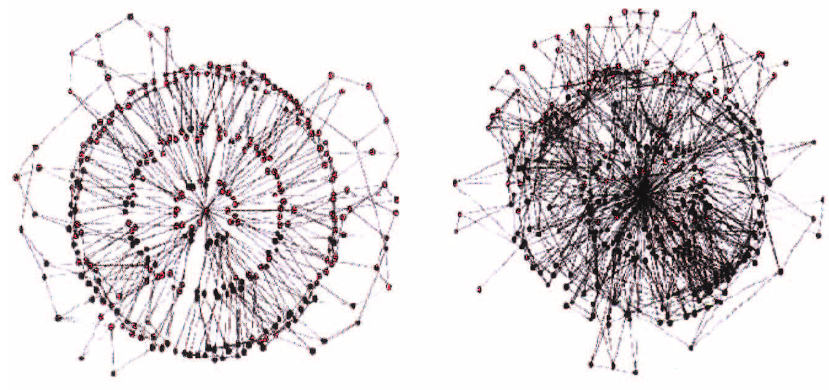
\includegraphics[width=150pt]{img/sample.png}}
%    \end{center}
%  \end{figure}
%\end{frame}
%%
%%
%\begin{frame}{Random Graphs}
%  \begin{itemize}
%    \item Formul\ae\\
%    \item \red{p}$*$\red{$N_1$}$*$(\red{N} - 1) / 2 connections
%  \end{itemize}
%\end{frame}
%%
%%
%\begin{frame}{SampleCode}
%We used the \red{peersim} library\footnote{\tiny{http://peersim.sourceforge.net/}} 
%  \begin{samplecode}
%    \begin{small}
%      // Generate a graph with an average of \red{k} connections\newline
%      // per node and randomness \red{r}\newline
%      Graph g = GraphFactory.wireKOut(g, k, r);\newline
%    \end{small}
%  \end{samplecode}
%\end{frame}
%%
%%
%\begin{frame}{SampleCode2}
%  \begin{samplecode}
%    \begin{tiny}
%      \begin{tabbing}
%        @WebService() \= public class \red{GraphService} \{\\
%        \> @WebMethod() public int [] \red{countNeighbours} (@WebParam() int [] adjVector) \{...\}\\
%        \> @WebMethod() public String [] \red{processConnections} (@WebParam() int [] neighboursCount) \{ ... \}\\
%        \> @WebMethod() \= public int [] \red{computeHops} ( @WebParam() int [] adjVector, \\
%        \> \> @WebParam() int [] neighbourCount,\\
%        \> \> @WebParam() int hyperNodeIndex) \{ ... \}\\
%        \}
%      \end{tabbing}
%    \end{tiny}
%  \end{samplecode}
%\end{frame}
%%
%

%----------------------------- PLY features
%
%% ``Outsider slide''
%
\section{Propylene}
\subsection{Overview}
%------------------------------
\begin{frame}{Propylene Design Goals}  


\end{frame}
%------------------------------




%\subsection{}
%%------------------------------
%\begin{frame}[label=2]{}
%  %
%  \begin{itemize}
%    \item
%\N
%    \item
%\N\N
%    \item 
%\N
%    \item
% 
%  \end{itemize}
%  %
%%
%\N\N
%\end{frame}



%----------------------------- Propylene description
\section{Propylene}

\subsection{Overview}
%------------------------------
\begin{frame}{Propylene architecture}
  %%
  Propylene is made of several stand-alone modules:
  %%
  \begin{figure}[!h]
    \begin{center}
      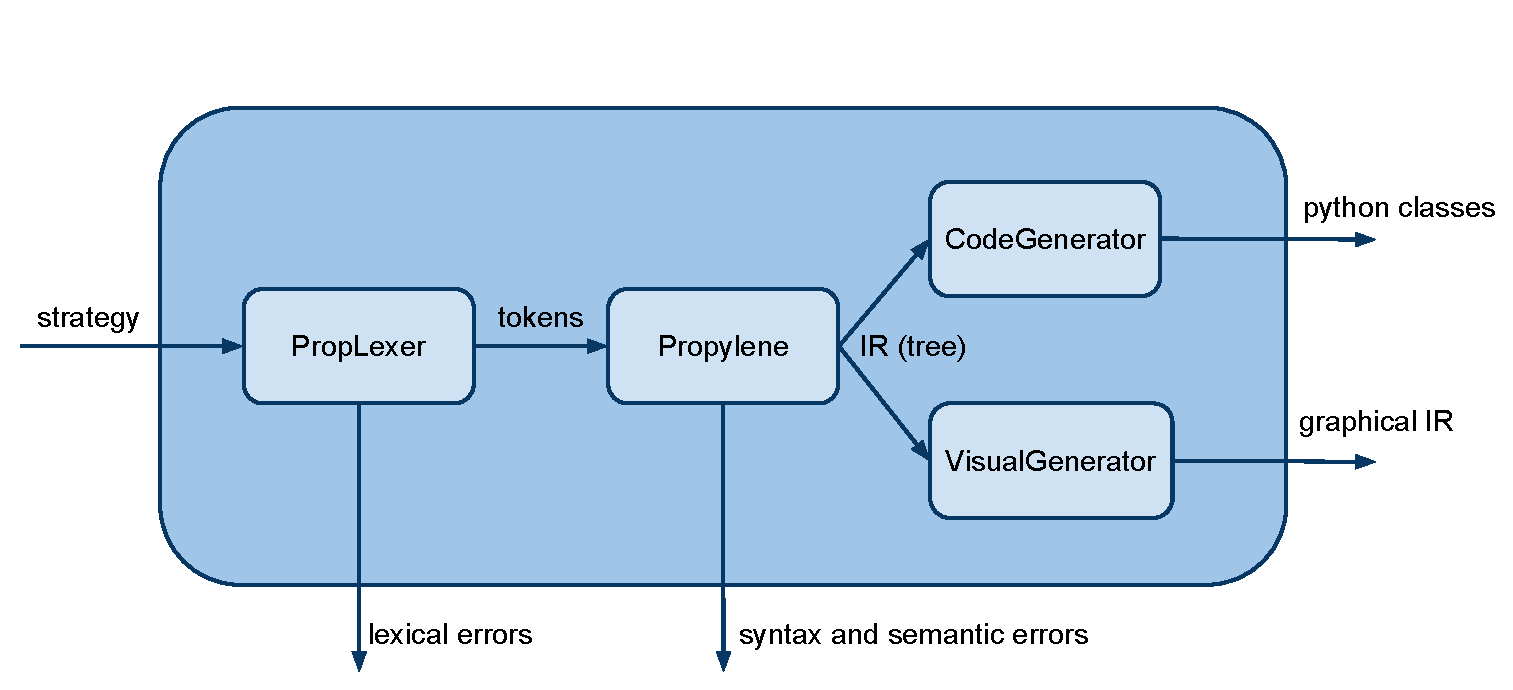
\includegraphics[width=300pt]{img/propylene.pdf}
    \end{center}
  \end{figure}
  %%
  Internally, it implements a \green{symbol table}.
  %%
\end{frame}


\subsection{AST}
%------------------------------
\begin{frame}{AST}  
  %
  %% \begin{itemize}
  %% \item Info concerning AST generation and traversal
  %%   \N
  %% \item Could contain some notes on Node hierarchy or Visitor
  %%   \N
  %% \item More...
  %%   \N
  %% \item AST Graphics here??
    
  %% \end{itemize}
  %
%
\N\N
\end{frame}



\subsection{Error Handling}
%------------------------------
\begin{frame}[fragile]{Syntax Errors}
  %
  \begin{itemize}
    \item \navy{Propylene} attempts to recover from erroneous input 
    by using its error rules
\n
    \item When the encountered syntax errors exceed a threshold, 
    the parser stop
\n
    \item The user will be notified with info related to all errors
    
  \end{itemize}
  %
\N
%%
  \begin{exampleblock}{Error Messages Example}
\begin{verbatim}
Line 14: Syntax error - unexpected token `)'
Line 14: Illegal Triggering Event
Line 17: Error detected in the Condition of the plan
Line 96: Error detected in the Body of the plan
\end{verbatim}
  \end{exampleblock}
%%
%
\N\N
\end{frame}


%------------------------------
\begin{frame}[fragile]{Semantic Errors}
  %
  \begin{itemize}
    \item \navy{Propylene} is able to identify two types of semantic errors:
\n
  %
  \begin{enumerate}
    \item Unbounded Variable \\
\n
    %%
    \texttt {
        ( +\tildett deposit\_corns() | ( white\_corn(\_("Y")))) >>\\ 
        \tab [ +\tildett grab\_corn(\_("X")) \#ERROR! ]
            }
    %%
\N
    \item Attitude Type Mismatch \\
\n
    %%
    \texttt {
        ( +\tildett deposit\_corns() ) >>\\ 
            \tab [ +\tildett grab\_corn("c11") \\
            \tab \tab deposit\_corns() \#ERROR! ]
            }
    %%

  \end{enumerate}
  %
\n
  \item In both cases, the parser stops immediately and notifies the user
  about the encountered error
  \end{itemize}
  %
%
\N\N
\end{frame}


\subsection{Graphics}
%------------------------------
\begin{frame}{Graphics}
  %
  \begin{itemize}
    \item Tree graphics, diagrams
\N
    \item final remarks
%\N
%    \item 
%\N
%    \item
% 
  \end{itemize}
  %
%
\N\N
\end{frame}







%\subsection{}
%%------------------------------
%\begin{frame}{}
%  %
%  \begin{itemize}
%    \item
%\N
%    \item
%\N
%    \item 
%\N
%    \item
% 
%  \end{itemize}
%  %
%%
%\N\N
%\end{frame}



%----------------------------- Case study (not useful)
%\include{casestudy}


\section{Conclusions}
%
\begin{frame}{Conclusions}
% 3 final remarks
  \begin{itemize}
    \item \navy{Propylene} is a Python classes generator that extracts
    \textbf{Profeta Attitudes} from \textbf{Profeta Plans}
\N
    \item \navy{Propylene} uses a pure-Python implementation of \textbf{lex}
    and \textbf{yacc}, \red{PLY}, as parsing tools
\N
    \item \navy{Propylene} provides a \textbf{graphical representation} 
    of the parse tree that is used to generate the code
  \end{itemize}
\end{frame}
%
%
%
\end{document}
